\documentclass{beamer}
\usepackage[utf8]{inputenc}

\usepackage{utopia} %font utopia imported
\usepackage{amsmath}
\usepackage{amsfonts}
\usepackage{amssymb}
\usepackage{graphicx}
\usetheme{Edinburgh}
\usepackage[cache=true]{minted}
\usemintedstyle{friendly}
\newenvironment{code}{\VerbatimEnvironment\begin{minted}{python}}{\end{minted}}
\newcommand{\icode}[1]{\mintinline{python}{#1}}  % inline code
\usecolortheme{default}
\usepackage{hyperref}
\hypersetup{
    colorlinks = true,
    linkcolor=blue
}


\title{Accelerate Python with Numba}

\subtitle{A Quick Introduction}

\author{Haoran Peng}


\date{Edinburgh Cohort Meeting, 17 August 2020}



\logo{
\includegraphics[height=1cm]{eushield-normal.png}}


\AtBeginSection[]
{
  \begin{frame}
    \frametitle{Table of Contents}
    \tableofcontents[currentsection]
  \end{frame}
}
%------------------------------------------------------------


\begin{document}

%The next statement creates the title page.
\frame{\titlepage}


%---------------------------------------------------------
%This block of code is for the table of contents after
%the title page
\begin{frame}
\frametitle{Table of Contents}
\tableofcontents
\end{frame}
%---------------------------------------------------------
\section{Numba Overview}

\begin{frame}
\frametitle{What is Numba?}
Here is the description from \href{http://numba.pydata.org/}{Numba's website}:
\begin{figure}
\centering
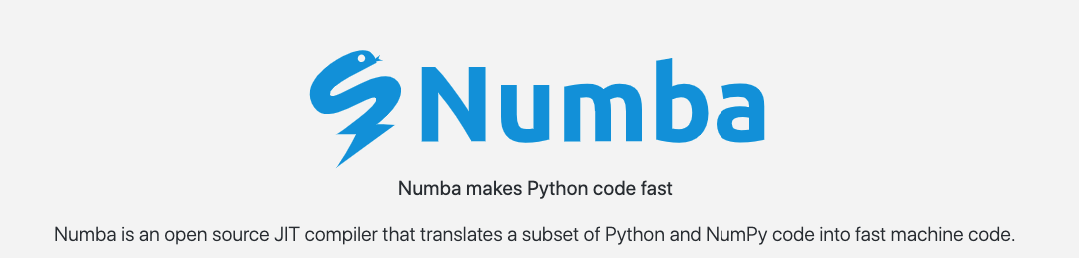
\includegraphics[width=\textwidth]{numba-official}
\end{figure}\pause
\begin{itemize}
\item<1-> Compiles Python code just-in-time (JIT)
\item<3-> Supports a subset of Python and NumPy
\item<4-> Translates directly to machine code
\end{itemize}
\end{frame}

\begin{frame}[fragile]
\frametitle{Toy (Unfair) Example: Sum from 1 to $N$}
\begin{columns}
\column{0.5\textwidth}
\begin{code}
def sum_py(n):
    ans = 0
    for i in range(1, n+1):
        ans += i
    return ans
\end{code}

\pause

\column{0.5\textwidth}
\begin{code}
from numba import jit

@jit
def sum_nb(n):
    ans = 0
    for i in range(1, n+1):
        ans += i
    return ans
\end{code}
\end{columns}
\end{frame}


\section{Why acceleration?}

\begin{frame}
\frametitle{Premature Optimization is the Root of All Evil}
I am doing a project on constituency parsing and need to use the \href{https://en.wikipedia.org/wiki/CYK_algorithm}{CYK algorithm}.
\vspace*{0.3cm}

You don't need to know the details about CYK, it is just a dynamic programming algorithm with  $O(n^3|G|)$ complexity, i.e. 3 for loops.
\vspace*{0.3cm}

{\footnotesize $n$ is the length of the sentence to be parsed.

$|G|$ is the size of the grammar.} \vspace*{0.3cm}\pause

\begin{figure}
\centering
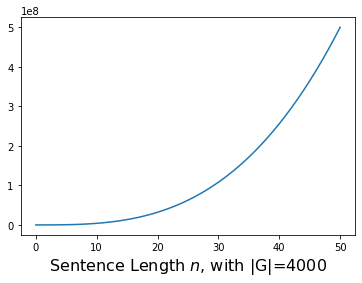
\includegraphics[width=.4\textwidth]{n3G}
\end{figure}

Parsing \textbf{cannot be done in reasonable time} using pure Python. 
\end{frame}

\begin{frame}[fragile]
\frametitle{Code to Accelerate}
We are going to tackle the edit distance problem which is very hard for the compiler to optimise:  

\begin{minted}[fontsize=\footnotesize]{python}
def edit_dist(s , t):
        m, n = len(s), len(t)
        dp = [[0]*(n + 1) for _ in range(m + 1)]
        for i in range(m + 1):
            dp[i][0] = i 
        for j in range(n + 1):
            dp[0][j] = j
        for i in range(1, m + 1):
            for j in range(1, n + 1):
                if s[i - 1] == t[j - 1]:
                    substitution_cost = 0
                else:
                    substitution_cost = 1
                dp[i][j] = min(dp[i - 1][j] + 1,
                               dp[i][j - 1] + 1,
                               dp[i - 1][j - 1] + substitution_cost)
        return dp[m][n]
\end{minted}
\end{frame}

\begin{frame}
\begin{figure}
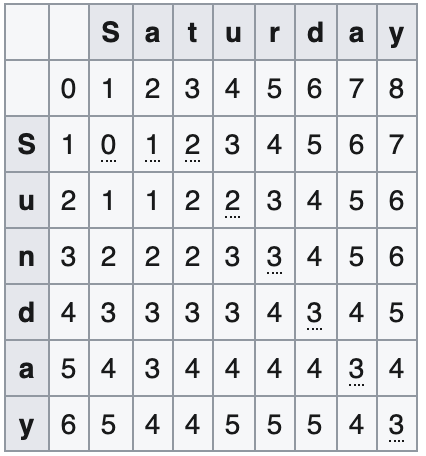
\includegraphics[width=.5\textwidth]{edit-dist}
\end{figure}
\footnotesize Image taken from \href{https://en.wikipedia.org/wiki/Levenshtein_distance}{Wikipedia}.
\end{frame}

\section{Accelerate step-by-step}
\begin{frame}
\frametitle{\icode{@jit(nopython=True)} and \icode{@njit}}
It would be nice if we can just \icode{@jit} every function and it would magically run much faster, but it isn't the case. \vspace*{0.3cm}\pause

Use \icode{@njit} only, because we don't want our ``accelerated" code to run slower. \vspace*{0.3cm}\pause

Although you can call into the Python interpreter in nopython mode using the \href{https://numba.pydata.org/numba-doc/latest/user/withobjmode.html?highlight=interpreter}{\icode{objmode} context-manager} (currently experimental).
\end{frame}

\begin{frame}
\frametitle{Re-write Unsupported Functions}
Numba only supports a subset of Python and NumPy, thus it is usually necessary to re-write some functions for \icode{@njit} to work. \vspace*{0.3cm} \pause

Though our edit distance code can be \icode{@njit}:ed directly.\footnote{As of 15/08/2020 when reflected list is still supported.}
\end{frame}

\begin{frame}
\frametitle{Use NumPy Arrays Instead of List if Possible}
NumPy arrays are contiguous in memory, thus much faster to access. Use them instead of lists if your problem permit you to do so. \vspace*{0.3cm} \pause

Most of the basic NumPy operations are supported in Numba.
\end{frame}

\begin{frame}
\frametitle{Performance Comparison}
\begin{figure}
\centering
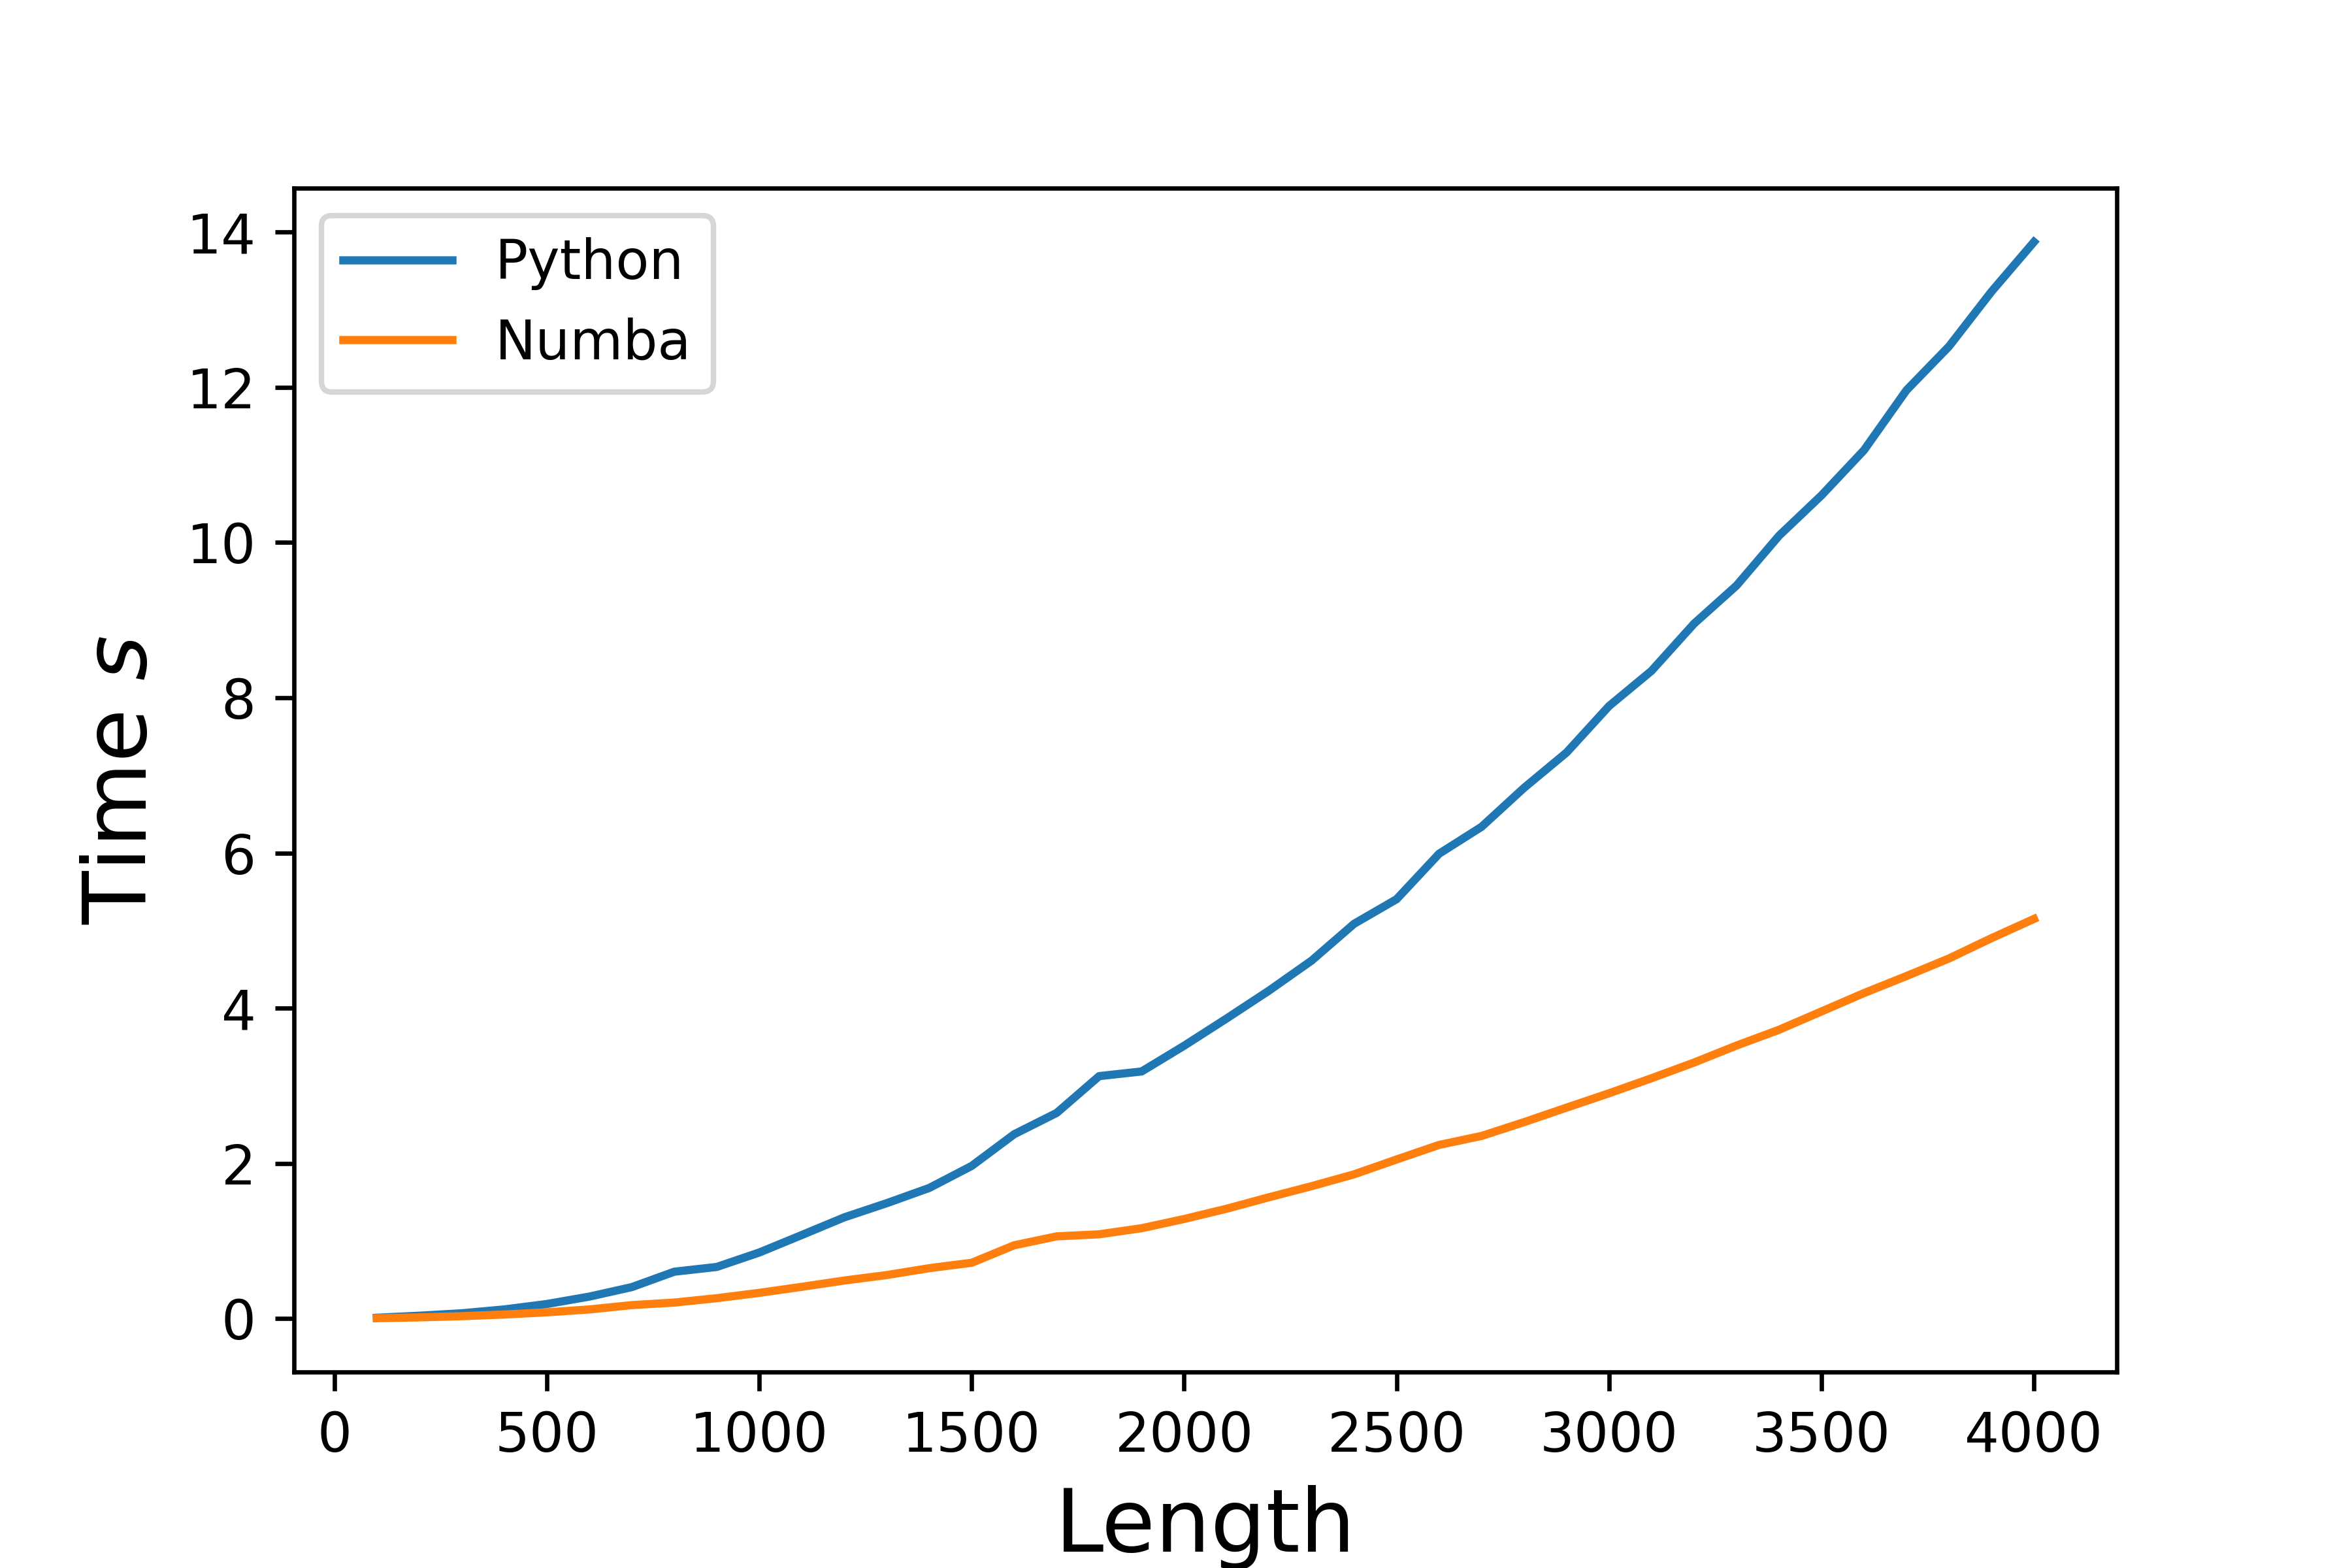
\includegraphics[width=.8\textwidth]{py_nb}
\end{figure}
\end{frame}

\begin{frame}
\frametitle{Use Typed Data Structures}
Python (reflected) list in jitted function will be deprecated soon. Replace the list with a Numba typed-list. \vspace*{0.3cm}\pause

Numba also has typed-dictionaries and (soon) typed-sets. 
\end{frame}

\begin{frame}
\frametitle{Multi-threading with \icode{@njit(nogil=True)}}
Because Numba code is compiled and does not depend on the Python interpreter, it can give up the GIL when executing. This makes (real) multi-threading possible in Python.
\end{frame}

\begin{frame}
\frametitle{Multi-threading with \icode{numba.prange}}
The same multi-threading can often be achieved by using Numba's \icode{prange} function. It automatically threads each iteration of the loop. But you give up some control by doing so.
\end{frame}

\section{Conclusion}
\begin{frame}
\frametitle{What more?}
\begin{itemize}
\item<1-> Automatic nested threading using OpenMP/TBB.
\item<2-> Optimization according to your architecture with LLVM.
\item<3-> GPU/cuda support, can manipulate array-like objects as long as they implement \icode{__cuda_array_interface__}.
\item<4-> Go check out \href{https://numba.pydata.org/numba-doc/latest/reference/index.html}{Numba's reference manual}, it's fairly well-written.
\end{itemize}


\end{frame}
\begin{frame}
\frametitle{Current Python Acceleration Landscape}
\begin{itemize}
\item<1-> Numpy, PyTorch, Tensorflow 
\item<2-> Cython, Numba
\item<3-> PyPy
\end{itemize}
\end{frame}
\end{document}